% Template created by Karol Kozioł (www.karol-koziol.net) for ShareLaTeX

\documentclass[a4paper,9pt]{extarticle}
\usepackage[utf8]{inputenc}
\usepackage[T1]{fontenc}
\usepackage{graphicx}
\usepackage[x11names]{xcolor}
\usepackage{tikz}
\usepackage{fontawesome5}
\usepackage{bm}
\usepackage[most]{tcolorbox}
\usepackage{enumerate}
\usepackage[shortlabels]{enumitem}
\tcbuselibrary{skins,raster,theorems,breakable}

\usepackage{amsmath,amssymb,textcomp}
\usepackage{mathtools}
\everymath{\displaystyle}
\usepackage{multicol}
\usepackage{multirow}
\setlength{\columnseprule}{0pt}
\setlength{\columnsep}{20.0pt}


\usepackage{geometry}
\geometry{a4paper,left=10mm,right=10mm,top=10mm,bottom=15mm}

\newcommand{\trans}[1]{{#1}^{\mathsf{T}}}
\newcommand{\ev}[1]{\mathbb{E}\left[#1\right]}
\newcommand{\unmezz}{\frac{1}{2}}

\newtcolorbox{riquadro}[1][]{enhanced, breakable,frame style={top color=Aquamarine3,bottom color=Aquamarine3},colback=black!80,coltext=Aquamarine3!50,title=#1,fonttitle=\bfseries,halign title=center,coltitle=black!80}
\makeatletter
\renewcommand*{\maketitle}{%
	\noindent
	\begin{minipage}{0.4\textwidth}
		
\begin{tikzpicture}
			\node[rectangle,rounded corners=6pt,inner sep=10pt,fill=SteelBlue4,text width= 0.95\textwidth] {\color{white}\Huge \@title};
		\end{tikzpicture}
	\end{minipage}
	\hfill
	\begin{minipage}{0.55\textwidth}
		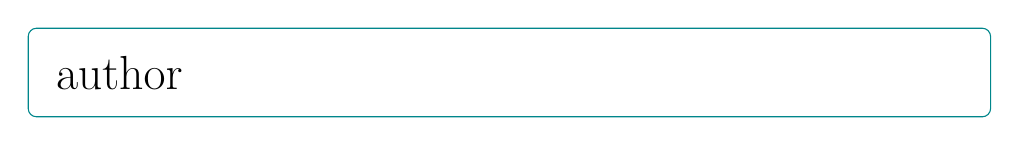
\begin{tikzpicture}
			\node[rectangle,rounded corners=3pt,inner sep=10pt,draw=Turquoise4,text width= 0.95\textwidth] {\LARGE \@author};
		\end{tikzpicture}
	\end{minipage}
}%
\makeatother
\newtcbtheorem[number within=section]{myproof}{Proof}{
	enhanced, sharp corners, breakable,
	colframe=LightSalmon1, coltitle=black, colbacktitle=gray!24,
	coltext=LightSalmon1!60,
	colback=black!80,
	rounded corners,
	fonttitle=\bfseries,
	separator sign={:},
	theorem hanging indent/.try=0pt,
}{ciao}

% custom section
\usepackage[explicit]{titlesec}
\newcommand*\sectionlabel{}
\newcommand{\pr}{\mathbb{P}}
\newcommand{\mbf}[1]{\mathbf{#1}}

\titleformat{\section}
{\gdef\sectionlabel{}
	\normalfont\rmfamily\Large\bfseries}
{\gdef\sectionlabel{\thesection\ }}{0pt}
{
	\noindent
	\begin{tikzpicture}
		\node[rectangle,rounded corners=3pt,inner sep=4pt,fill=Turquoise4,text width= 0.95\columnwidth] {\color{white}\sectionlabel#1};
	\end{tikzpicture}
}
\titlespacing*{\section}{0pt}{0pt}{-10pt}
\newcommand*\subsectionlabel{}
\titleformat{\subsection}
{\gdef\subsectionlabel{}
	\normalfont\rmfamily\Large\bfseries}
{\gdef\subsectionlabel{\thesubsection\ }}{0pt}
{
	\noindent
	\begin{tikzpicture}
		\node[rectangle,inner sep=4pt,fill=Turquoise4!60!black,rounded corners=3pt,text width= 0.9\columnwidth] {\color{white}\subsectionlabel#1};
	\end{tikzpicture}
}
\titlespacing*{\subsection}{0pt}{0pt}{0pt}

% custom footer
\usepackage{fancyhdr}
\makeatletter
\pagestyle{fancy}
\fancyhead{}
\fancyfoot[C]{\footnotesize \textcopyright\ \@date\ \ \@author}
\renewcommand{\headrulewidth}{0pt}
\renewcommand{\footrulewidth}{0pt}
\makeatother



\title{Il Diocane: Introduction to Data Mining Cheatsheet}
\author{\faSynagogue\;Kotatsu, the Bringer of Jewishness\;\faMenorah}
\date{\today}



\begin{document}
	
\maketitle
	
\begin{multicols*}{2}
\section{Similarity and dissimilarity}
\begin{riquadro}
	Entropy:
	\begin{equation*}
		H(X)=-\sum_{i=1}^{n}p_{i}\log_{2}p_i.
	\end{equation*}
	Sample entropy:
	\begin{equation*}
		H(X)=-\sum_{i=1}^{n}\frac{m_{i}}{m}\log_{2}\frac{m_{i}}{m}
	\end{equation*}
	Mutual information:
	\begin{equation*}
		I(X,Y)=H(X)+H(X)-H(X,Y)
	\end{equation*}
	where $H(X,Y)=-\sum_{i=1}^{n}\sum_{j=1}^{n}p_{ij}\log_{2}p_{ij}$. For discrete variables the maximum mutual information is 
	\begin{equation*}
		\log_{2}(\min\{n_{x},n_{y}\})
	\end{equation*}
	where $n_{x}$ is th number of values that $X$ can take.
\end{riquadro}
We can combine similarities with
\begin{equation*}
	\mathrm{similarity}(\mathbf{x},\mathbf{y})=\frac{\sum_{k=1}^{n}w_k\delta_{k}s_{k}((\mathbf{x},\mathbf{y}))}{\sum_{k=1}^{n}w_k\delta_{k}}
\end{equation*}
with
\begin{equation*}
	\delta_{k}=\begin{cases}
		0&\text{\footnotesize\parbox{2.5cm}{if both attribute are asymmetric AND they are both zero or if one of them is missing}}\\
		1&\text{\footnotesize otherwise}
	\end{cases}
\end{equation*}
\section{Clustering}
\begin{riquadro}
	Number of possible clusters:
	\begin{equation*}
		B(n)=\sum_{k=0}^{\infty}\frac{k^{n}}{k!}
	\end{equation*}
	Sum of squared error (what we want to minimize):
	\begin{equation*}
		\mathrm{SSE}=\sum_{i-1}^{K}\sum_{x\in C_i}\mathsf{dist}(m_i,x)^{2}.
	\end{equation*}
\end{riquadro}
So we are trying to minimize the loss function, for the centroids of $K$ clusters $\mathbf{c}=(c_1,\ldots,c_K)$:
\begin{equation*}
	\mathrm{L}(\mathbf{c})=\sum_{i=1}^{n}\min_{j=1,\ldots,K}\lVert x_{i}-c_{j}\rVert^{2}_{2}.
\end{equation*}
We alternate between
\begin{itemize}
	\item updating $z_{i}=\arg\min_{j=1,\ldots,k}\lVert x_{i}-c_{j}\rVert^{2}_{2}$ (maps point $x_{i}$ to a cluster j);
	\item updating $c_{j}=\frac{1}{\left|\{i|z_{i}=j\}\right|}\sum_{i|z_{i}=j}x_{i}$ (recomputes the cluster centroids)
\end{itemize}
\begin{riquadro}[Unsupervised measures of cluster validity]
	\begin{itemize}
	\item 	\textbf{Cohesion}: within-cluster sum of squares (SSW)
	\begin{equation*}
		\mathrm{SSW}=\sum_{i=1}^{K}\sum_{x\in C_i}(x-m_{i})^{2}.
	\end{equation*}
	\item \textbf{Separation}: between-cluster sum of squares (SSB)\\
	\begin{equation*}
		\mathrm{SSB}=\sum_{i}|C_{i}|(m-m_i)^{2}
	\end{equation*}
	where $|C_{i}|$ is the size of cluster $i$ and $m$ is the global centroid.\\
	\item \textbf{Silhouette coefficient}: for a point $P_{i}$ calculate the avg distance $a$ to the points of the cluster and the minimum avg distance $b$ to the points of another cluster. The silhouette coefficient is
	\begin{equation*}
		s=\frac{b-a}{\max\{a,b\}}.
	\end{equation*}
	\end{itemize}
\end{riquadro}
\begin{riquadro}[Supervised measures of cluster validity]
	\begin{itemize}
	\item 	\textbf{Label probability per cluster}:
	\begin{equation*}
		p_{ij}=\frac{m_{ij}}{m_{j}}
	\end{equation*}
	where $m_{j}$: size of cluster $j$ and $m_{ij}$: number of elements of cluster $j$ that are labelled $i$.
	\item \textbf{Entropy of cluster $j$}:
	\begin{equation*}
		h_{j}=\sum_{i=1}^{L}p_{ij}\log_{2}p_{ij}.
	\end{equation*}
\textbf{Total entropy}:
	\begin{equation*}
		h=\sum_{j=1}^{K}\frac{m_{j}}{m}h_{j}.
	\end{equation*}
	\item \textbf{Purity}:
	\begin{equation*}
		\mathrm{purity}_{j}=\max\{p_{ij}\}.
	\end{equation*}
	\textbf{Total purity}:
	\begin{equation*}
		\mathrm{purity}=\sum_{j=1}^{K}\frac{m_{j}}{m}\mathrm{purity}_{j}.
	\end{equation*}
	\item \textbf{Precision}:
	\begin{equation*}
		\frac{TP}{TP+FP}=\frac{m_{ij}}{m_{j}}=p_{ij}.
	\end{equation*}
	\item \textbf{Recall}:
	\begin{equation*}
		\frac{TP}{TP+FN}=\frac{m_{ij}}{m_{i}}.
	\end{equation*}
	\item \textbf{F-measure}:
	\begin{equation*}
		2\cdot\frac{\text{precision}\cdot\text{recall}}{\text{precision}+\text{recall}}.
	\end{equation*}
	\end{itemize}
\end{riquadro}
	Remember that we have
\begin{center}
	\begin{tabular}{|c|c|cc|}
		\cline{3-4}
		\multicolumn{2}{c}{}&\multicolumn{2}{|c|}{cluster}\\
		\cline{3-4}
		\multicolumn{2}{c|}{}&same&different\\
		\hline
		\multirow{2}{*}{\rotatebox[origin=c]{90}{class\hspace*{0.5cm}}}&\rotatebox[origin=c]{90}{same}&$f_{11}$&$f_{10}$\\
		\cline{2-4}
		&\rotatebox[origin=c]{90}{different}&$f_{01}$&$f_{00}$\\
		\hline
	\end{tabular}
\end{center}
\begin{riquadro}[More supervised measures]
	\begin{itemize}
		\item \textbf{Rand statistic}:
		\begin{equation*}
			R=\frac{f_{00}+f_{11}}{f_{00}+f_{01}+f_{10}+f_{11}}.
		\end{equation*}
		\item \textbf{Jaccard coefficient}:
		\begin{equation*}
			J=\frac{f_{11}}{f_{01}+f_{10}+f_{11}}.
		\end{equation*}
		\item \textbf{Adjusted Rand Index}:
		\begin{equation*}
			\mathrm{ARI}=\frac{R(L,C)-\ev{R(L,C)}}{\max\left\{R(L,C),\ev{R(L,C)\right\}}}
		\end{equation*}
		with
		\begin{align*}
			\ev{R(L,C)}&=\frac{\pi(L)\pi(C)}{\frac{n(n-1)}{2}}\\
			\max\left\{R(L,C)\right\}&=\unmezz(\pi(L)-\pi(C))
		\end{align*}
		with $\pi(C)$: number of objects pairs that belong to the same group $C$.
	\end{itemize}
\end{riquadro}
\section{Fuzzy clustering}
We generalize $k$-mean objective function
\begin{equation*}
	\mathrm{SSE}=\sum_{j=1}^{k}\sum_{i=1}^{n}w_{ij}^{p}\mathrm{dist}\left(\mathbf{x}_{i},\mathbf{c}_{j}\right)^{2}.
\end{equation*}
So the procedure is
\begin{enumerate}
	\item choose random weights $w_{ij}$;
	\item until centroids do not change:
	\begin{enumerate}
		\item $\mathbf{c}_{j}=\frac{\sum_{i=1}^{n}w_{ij}\mathbf{x}_{i}}{\sum_{i=1}^{n}w_{ij}}$ (updates centroids);
		\item $w_{ij}=\frac{\left(\frac{1}{\mathrm{dist}(\mathbf{x_{i},\mathbf{c}_{j}})^{2}}\right)^{\frac{1}{p-1}}}{\sum_{q=1}^{k}\left(\frac{1}{\mathrm{dist}(\mathbf{x_{i},\mathbf{c}_{q}})^{2}}\right)^{\frac{1}{p-1}}}$ (updates weights).
	\end{enumerate}
\end{enumerate}
\section{Probabilistic clustering}
Model the set of data points as arising from a mixture of distributions. Each cluster corresponds to one distribution from the mixture. Clusters are found by estimating the parameters of the statistical distributions using Expectation-maximization algorithm.\par
The probability that the $j$-th distribution with parameter $\vartheta_{j}$ is chosen to generate an object $x_{i}$ belonging to one of $K$ clusters is given by the weight $w_{j}$. So
\begin{equation*}
	\pr(x|\Theta)=\sum_{j=1}^{K}w_{j}p_{j}(x|\vartheta_{j}).
\end{equation*}
If the $m$ objects are generated independently then
\begin{equation*}
	\pr(x|\Theta)=\prod_{i=1}^{m}\sum_{j=1}^{K}w_{j}p_{j}(x|\vartheta_{j}).
\end{equation*}
\begin{riquadro}[Probabilistic clustering]
	\begin{enumerate}
		\item Estimation: for each point compute its probability under each distribution 
		\begin{equation*}
			\pr(x_{i}|\vartheta_{j}).
		\end{equation*}
		\item Maximization: update the parameters.
	\end{enumerate}
\end{riquadro}
Estimation is similar to $k$-means. Weights are probabilities, they are not raised to a power and are calculated using Bayes:
\begin{equation*}
	p(C_{j}|x_{i})=\frac{p(x_{i}|C_{j})p(C_{j})}{\sum_{l=1}^{k}p(x_{i}|C_{l})p(C_{l})}.
\end{equation*}
We can estimate
\begin{equation*}
	p(C_{j})=\frac{1}{m}\sum_{m}^{1}p(C_{j}|x_{i}).
\end{equation*}
Maximization step:
\begin{equation*}
	c_{j}=\frac{\sum_{i=1}^{m}x_{i}p(C_{j}|x_{i})}{\sum_{i=1}^{m}p(C_{j}|x_{i})}.
\end{equation*}
Complexity: $\mathcal{O}(d^{2})$.
\subsection{Density based algorithms}
\begin{riquadro}[Grid based clustering]
	\begin{enumerate}
		\item Define a set of grid cells.
		\item Assign objects to the appropriate cells and compute the density of each cell.
		\item Eliminate cells having a density below a specified threshold.
		\item Form clusters from continuous groups of dense cells.
	\end{enumerate}
\end{riquadro}
Complexity: $\mathcal{O}(n \log n)$.\par
The CLIQUE algorithm is based on the apriori principle: 
\begin{equation*}
	\begin{array}{c}
		\text{cluster in $k$}\implies\text{cluster in subsets of $k$}\\
		\text{no cluster in $k$}\implies\text{no cluster in supersets of $k$}
	\end{array}
\end{equation*}
\begin{riquadro}[CLIQUE]
	\begin{enumerate}
		\item Find all dense areas in the one-dimensional spaces corresponding to each attribute. This is the set of dense one-dimensional cells.
		\item $k\leftarrow2$.
		\item Until there are no candidate dense $k$-dimensional cells iterate:
		\begin{enumerate}
			\item Generate all candidate dense $k$-dimensional cells from dense $(k-1)$ dimensional cells.
			\item Eliminate cells that have fewer than $\tau$ points.
			\item $k\rightarrow k+1$.
		\end{enumerate}
		\item Find clusters by taking the union of all adjacent high density cells.
		\item Summarise each cluster using a small set of inequalities that describe the attribute ranges of the cells in the cluster.
	\end{enumerate}
\end{riquadro}
Time complexity: exponential.
\subsection{Graph-based clustering: chameleon}
Three steps:
\begin{enumerate}
	\item Sparsification of the proximity graph modifying the proximity matrix (can be recursive).
	\item Partitioning into a large number of roughly equally sized groups (ise METIS).
	\item Merging the large number of roughly equally sized groups (agglomerative hierarchical clustering based on dynamic modelling).
\end{enumerate}
Example of merging schemes: MIN (minimum distance between clusters) or GROUP-AVERAGE (avg connectivity). Dynamic modeling: adapt to the characteristics of the data set.
\begin{riquadro}[Dynamic modeling measures]
	Relative interconnectivity:
	\begin{equation*}
		\mathrm{RI}(C_{i},C_{j})=\frac{\mathrm{EC}(C_{i},C_{j})}{\unmezz\left(\mathrm{EC}(C_{i})+\mathrm{EC}(C_{j})\right)}.
	\end{equation*}
	Relative closeness:
	\begin{equation*}
		\mathrm{RC}(C_{i},C_{j})=\frac{\overline{S}_{\mathrm{EC}}(C_{i},C_{j})}{\frac{m_{i}}{m_{i}+m_{j}}\overline{S}_{\mathrm{EC}}(C_{i})+\frac{m_{j}}{m_{i}+m_{j}}\overline{S}_{\mathrm{EC}}(C_{j})}
	\end{equation*}
\end{riquadro} 
For example: \begin{itemize}
	\item combine pair of clusters which maximises $\mathrm{RI}\times \mathrm{RC}^{\alpha}$ and stop when there are $K$ clusters left;
	\item combine clusters which have $\mathrm{RC}>t_{c}$ and $\mathrm{RC}>t_{i}$.
\end{itemize}
\subsection{Spectral clustering}
Given a proximity matrix $\mathbf{W}$ (weighted adjacency matrix) define a diagonal matrix $\mathbf{D}$ such that
\begin{equation*}
	D_{ij}=\begin{cases}
		\sum_{l}W_{il}&\text{if }i=j\\
		0&\text{otherwise.}
	\end{cases}
\end{equation*}
Compute the laplacian
\begin{equation*}
	\mathbf{L}=\mathbf{D}-\mathbf{W}.
\end{equation*}
We have that $\mathbf{L}$ is symmetric, positive semidefinite and all eigenvalues are positive for any vector $\mathbf{v}$:
\begin{equation*}
	\trans{\mathbf{v}}\mathbf{L}\mathbf{v}\geq 0.
\end{equation*}
Write $\mbf{L}$ as eigenvalue decomposition:
\begin{equation*}
	\mbf{L}=\mbf{\Lambda}\mbf{V}.
\end{equation*}
\begin{riquadro}[Spectral clustering]
	\begin{enumerate}
		\item Create a sparsified similarity graph.
		\item Compute the laplacian.
		\item Create a matrix $\mbf{V}$ from the first $k$ eigenvalues of $\mbf{L}$.
		\item Apply $k$-means on $\mbf{V}$.
	\end{enumerate}
\end{riquadro}
\subsection{SNN Clustering}
\begin{riquadro}[SNN Algorithm]
	\begin{enumerate}
		\item Compute similarity matrix.
		\item Sparsify the similarity matrix (keep only $k$ most similar neighbours).
		\item Construct the SNN graph from the sparsified similarity matrix.
		\item Find the SNN density of each point.
		\item Find the core points using parameter \textit{MinPts}.
		\item For clusters from the core points.
		\item Discard all noise points.
		\item Assign all non noise, non core points to clusters.
	\end{enumerate}
	Steps 4-8 are DBSCAN.
\end{riquadro}
\section{Anomaly detection}
We can have:
\begin{itemize}
	\item statistical approaches;
	\item distance-based approaches (from the object to its $k$-th nearest neighbor);
	\item density-based approaches: different density measures possible:
	\begin{equation*}
		\mathrm{density}(x,k)=\frac{1}{K_{\mathrm{dist}}}.
	\end{equation*} Relative density:
	\begin{align*}
		\mathrm{rel\_dens}(x,k)&=\frac{\sum_{i=1}^{k}\frac{\mathrm{density}(y_{i},k)}{k}}{\mathrm{density}(x,k)}\\
		&=\frac{K_{\mathrm{dist}}(x,k)}{\frac{\sum_{i=1}^{k}K_{\mathrm{dist}}(y_{i},k)}{k}}.
	\end{align*}
	You can use reachability distance
	\begin{equation*}
		R^{K}_{\mathrm{dist}}(x,y_{1})=\max\left\{K_{\mathrm{dist}}(y_{1}),\mathrm{dist}(x,y_{1})\right\}.
	\end{equation*}
	\begin{riquadro}[LOF algorithm]
		\begin{enumerate}
			\item Compute the local reachability density of $x$ as inverse of avg reachability distance:
			\begin{equation*}
				L^{K}_{\mathrm{density}}(x)=\frac{1}{\left(\frac{\sum_{y\in N_{K}(x)}R^{K}_{\mathrm{dist}}(X,y)}{|N_{K}(x)|}\right)}.
			\end{equation*}
			\item Relate it to the one of the neighbours:
			\begin{equation*}
				\mathrm{LOF}_{K}(x)=\frac{\sum_{y\in N_{K}(x)}L^{K}_{\mathrm{density}}(y)}{|N_{K}(x)|}\frac{1}{L^{K}_{\mathrm{density}}(x)}
			\end{equation*}
		\end{enumerate}
	\end{riquadro}
	Complexity is $\mathcal{O}(n^{2})$;
	\item clustering-based approaches:
	\begin{itemize}
		\item prototype based clusters;
		\item density based clusters;
		\item graph based clusters;
	\end{itemize}
	\item reconstruction based approaches: use dimensionality reduction like PCA/autoencoders to project $x$ to $\hat{x}$ and define reconstruction error as
	\begin{equation*}
		\lVert x-\hat{x}\rVert.
	\end{equation*}
	Autoencoders minimize this. If this is high it is an anomaly;
	\item information theory approach: anomalies bring a decrease in information when they are deleted.
\end{itemize}
\section{Classification}
\subsection{Decision trees}
Many possible decision trees that can be built from the
same dataset. The goal of the learning algorithm is to find the best tree among all possible
trees.
\begin{riquadro}[Hunt's algorithm]
	\begin{enumerate}
		\item Check if the tree is pure: if yes create a leaf.
		\item Otherwise, split it according to the best condition.
		\item Add a new node in the decision tree and associate it with that condition.
		\item For each branch of the new node apply recursively the algorithm.
	\end{enumerate}
\end{riquadro}
Continuous attributes need binning. We prefer nodes with purer class distributions. Measures of impurity of a node $t$ ($p_{c}(t)$: frequency of class $c$ at node $t$ over total number of classes $C$):
\begin{itemize}
	\item Gini index:
	\begin{equation*}
		1-\sum_{c=1}^{C}p_{c}(t)^{2};
	\end{equation*}
	when a node is split the Gini index for the split is the weighted average of the Gini index evaluated on the resulting nodes:
	\begin{equation*}
		\sum_{k=1}^{K}\frac{n_{k}}{n}\mathrm{Gini}(t_{k})
	\end{equation*}
	where $n_{k}$ is the number of examples in the $k$-th split node;
	\item Entropy:
	\begin{equation*}
		-\sum_{c=1}^{C}p_{c}(t)\log_{2}p_{c}(t);
	\end{equation*}
	after splitting we have
	\begin{equation*}
		\mathrm{Entropy}(t_{parent})-\sum_{k=1}^{K}\frac{n_{k}}{n}\mathrm{Entropy}(t_{k});
	\end{equation*}
	\item Classification error:
	\begin{equation*}
		1-\max_{c}\left\{p_{c}(t)\right\}.
	\end{equation*}
\end{itemize}
Choose the attribute test condition that yields the lowest impurity score. To avoid too many partition define the gain ratio
\begin{equation*}
	\text{GainRation}=\frac{\text{InformationGain}}{-\sum_{k=1}^{K}\frac{n_{k}}{n}\log_{2}\frac{n_{k}}{n}}.
\end{equation*}
\subsection{Rule-based classification}
Uses a collection of if-then:
\begin{equation*}
	\text{Condition}_{i}=(A_{1}\odot v_{1})\wedge\ldots\wedge(A_{k}\odot v_{k}).
\end{equation*}
Coverage: fraction of instances that satisfy the rule's antecedent
\begin{equation*}
	\frac{|A|}{|D|}.
\end{equation*}
Accuracy: fraction of instances that satisfy the rule's antecedent and consequent
\begin{equation*}
	\frac{|A\cap y|}{|D|}.
\end{equation*}
Example: RIPPER.
\subsection{Naive Bayes}
We seek for the most probable hypothesis given the data and any initial knowledge about the prior probabilities. MAP hypothesis:
\begin{align*}
	h_{\mathrm{MAP}}&=\arg\max_{h\in\mathcal{H}}\pr(h|D)\\
	&=\arg\max_{h\in\mathcal{H}}\frac{\pr(D|h)\pr(h)}{\pr(D)}\\
	&=\arg\max_{h\in\mathcal{H}}\pr(D|h)\pr(h).
\end{align*}
If we assume that all hypotheses are equally likely a priori we can only consider the likelihood of the data (Maximum Likelihood hypothesis):
\begin{equation*}
	h_{\mathrm{ML}}=\arg\max_{h\in\mathcal{H}}\pr(D|h).
\end{equation*}
MDL principle:
\begin{align*}
		h_{\mathrm{MAP}}&=\arg\max_{h\in\mathcal{H}}\pr(D|h)\pr(h)\\
		&=\arg\max_{h\in\mathcal{H}}\log_{2}\pr(D|h)+\log_{2}\pr(h)\\
		&=\arg\min_{h\in\mathcal{H}}-\log_{2}\pr(D|h)-\log_{2}\pr(h).
\end{align*}
This is like minimizing the number of bits transmitted to encode the data and the hypothesis. Given a class $y_{i}\in\mathcal{Y}$ we get
\begin{equation*}
	\pr(y_{j}|D)=\sum_{h\in\mathcal{H}}\pr(y_{j}|h)\pr(h|D)
\end{equation*}
so the Bayes Optimal Classifier is
\begin{equation*}
	y_{\mathrm{Bayes}}=\arg\max_{y_{j}\in\mathcal{Y}}\sum_{h\in\mathcal{H}}\pr(y_{j}|h)\pr(h|D)
\end{equation*}
but we need to know the posterior of all hypotheses (often impossible).
\begin{riquadro}[Gibbs' algorithm]
	\begin{enumerate}
		\item Choose an hypothesis $h\in\mathcal{H}$ at random according to the posterior probability over $\mathcal{H}$, which is $\pr(h|D)$.
		\item Use $h$ to classify the new instance.
	\end{enumerate}
\end{riquadro}
The error is at most twice the one of the OBC.
The naive Bayes classifier makes the assumption that the attributes are conditionally independent given the class:
\begin{equation*}
	\pr(a_{1},\ldots,a_{d}|y_{j})=\prod_{i=1}^{d}\pr(a_{i}|y_{j})
\end{equation*}
so the NBC is
\begin{equation*}
	y_{\mathrm{NB}}=\arg\max_{y_{j}\in\mathcal{Y}}\pr(y_{j})\prod_{i=1}^{d}\pr(a_{i}|y_{i}).
\end{equation*}
Probability are empyrical. Use laplace smoothing or m-estimate
\begin{equation*}
	\hat{\pr}(a_{i}|y_{i})=\frac{n_{a_{i},y_{i}}+1}{n_{y_{j}}+|A_{i}|}.
\end{equation*}
\subsection{KNN}
It is a lazy learner. Classifies based on the closest datapoint.
\section{Model selection}
Generalization error in the case of trees:
\begin{equation*}
	\mathrm{err}_{\text{gen}}(T)=\mathrm{err}(T)+\alpha\frac{k}{N_{\text{train}}}
\end{equation*}
\begin{riquadro}[MDL principle]
	Length of the shortest message that allows to reconstruct the labels.
	\begin{equation*}
		\mathrm{MDL}(D,M)=\text{Cost}(D|M)+\alpha\times\text{Cost}(M).
	\end{equation*}
\end{riquadro}
We can either do pre-pruning or post-pruning until generalization error cannot be improved.
\begin{riquadro}[Population Risk]
	Risk of a hypothesis $h\in\mathcal{H}$ as
	\begin{equation*}
		R[h]=\mathbb{E}_{(\bm{x},y)\sim\mathcal{D}}\left[l(y,h(\bm{x}))\right]
	\end{equation*}
\end{riquadro}
\begin{riquadro}[Empirical risk]
	Given a dataset $T$ whe have
	\begin{equation*}
		\hat{R}_{T}[h]=\frac{1}{n}\sum_{(\bm{x},y)\in T}l(y,h(\bm{x})).
	\end{equation*}
\end{riquadro}
\section{SRM}
A given training set 
\begin{equation*}
	D=\left\{(x_{1},y_{1}),\ldots,(x_{n},y_{n})\right\}
\end{equation*}
is assumed to be drawn iid from a fixed and unknown distribution $p(x,y)$. We want to learn a function $h^{\star}$ such that $\forall(x_{i},y_{i})\in D,\;h^{\star}(x_{i})=y_{i}$ (small population risk). We use some learning algorithm $A$ which optimizes some performance measure $l$ of the model (like a loss function). Expected risk minimization:
\begin{align*}
	h^{\star}&=\arg\min_{h\in\mathcal{H}}R[h]\\
	&=\arg\min_{h\in\mathcal{H}}\mathbb{E}_{(x,y)\sim p(x,y)}\left[l(h(x),y)\right]
\end{align*}
We use the empirical mean
\begin{equation*}
	h^{\star}=\arg\min_{h\in\mathcal{H}}\frac{1}{n}\sum_{i=1}^{n}l(h(x_{i}),y_{i}).
\end{equation*}
So the generalization error is the sum of the error of the training set and the model complexity term
\begin{equation*}
	R[h]=\hat{R}_{D}[h]+\alpha\cdot\text{Complexity}(h).
\end{equation*}
\begin{riquadro}[VC dimension]
	The VC dimension of a hypothesis space $\mathcal{H}$ defined over an instance space $X$ is the size of the largest finite subset of $X$ shattered by $\mathcal{H}$.
	\begin{equation*}
		\mathrm{VC}(\mathcal{H})=\max_{S\subset X}|S|:S\text{ is shattered by }\mathcal{H}.
	\end{equation*}
\end{riquadro}
The upper bound of the true risk is
\begin{equation*}
	R[h^{\star}]\leq\hat{R}_{D}[h^{\star}]+\mathcal{O}\left(\sqrt{\frac{\mathrm{VC}(\mathcal{H})}{n}\log\left(\frac{n}{VC(\mathcal{H})}\right)-\frac{\log(\delta)}{n}}\right)
\end{equation*}
\section{SVM}
Functional margin:
\begin{equation*}
	\mu(x_{i})=y_{i}(w\cdot x_{i}-t)=y_{i}f(x)
\end{equation*}
Geometric margin:
\begin{equation*}
	\mu=\frac{1+t}{\lvert\lvert\bm{w}\rvert\rvert}-\frac{t-1}{\lvert\lvert\bm{w}\rvert\rvert}=\frac{2}{\lvert\lvert\bm{w}\rvert\rvert}
\end{equation*}
\begin{riquadro}[SVM optimization]
	\begin{align*}
		&\min_{\bm{w},t}\unmezz\lvert\lvert\bm{w}\rvert\rvert^{2}\\
		\text{s.t. }&y_{9}(\bm{w}\cdot\bm{x}_{i}-t)\geq 1;\quad\forall i:1\leq i\leq n.
	\end{align*}
	Dual problem:
	\begin{align*}
		&\min_{\alpha}-\unmezz\sum_{i=1}^{n}\sum_{j=1}^{n}\alpha_{i}\alpha_{j}y_{i}y_{j}\bm{x}_{i}\bm{x}_{j}+\sum_{i=1}^{n}\alpha_{i}\\
		\text{s.t. }&\alpha_{i}>0\\
		&\sum_{i=1}^{n}y_{i}\alpha_{i}=0
	\end{align*}
\begin{align*}
	&\min_{\bm{\alpha}}\mathbf{1}^{T}\bm{\alpha}-\unmezz\bm{\alpha}^{T}\bm{YXX}^{T}\bm{Y\alpha}\\
	\text{s.t. }&\bm{\alpha}\succeq0\\
	&\bm{y}^{T}\bm{\alpha}=0.
\end{align*}
\end{riquadro}
	Written in matrix form we get
\begin{align*}
	&\min_{\bm{\alpha}}\mathbf{1}^{T}\bm{\alpha}-\unmezz\bm{\alpha}^{T}\bm{YXX}^{T}\bm{Y\alpha}\\
	\text{s.t. }&\bm{\alpha}\succeq0\\
	&\bm{y}^{T}\bm{\alpha}=0.
\end{align*}
Introduce one slack variable for each training sample:
\begin{align*}
	&\min_{\bm{w},t,\xi}\unmezz\lvert\lvert\bm{w}\rvert\rvert^{2}+C\sum_{i=1}^{n}\xi_{i}\\
	\text{s.t.}&y_{i}(\bm{w}\cdot \bm{x}_{i}-t)\geq 1-\xi_{i}\qquad\forall1\leq i\leq n\\
	&\xi_{i}\geq0\qquad\forall1\leq i\leq n.
\end{align*}
Given a feature map $\phi$ we have 
\begin{equation*}
	\bm{w}=\sum_{i=1}^{n}\alpha_{i}y_{i}\phi(\bm{x}_{i})
\end{equation*}
and the decision function is
\begin{align*}
	f(\bm{x})&=\bm{w}\cdot\phi(\bm{x})-t\\
	&=\sum_{i=1}^{n}\alpha_{i}y_{i}\phi(\bm{x}_{i})\cdot\phi(\bm{x})-t\\
	&=\sum_{i=1}^{n}\alpha_{i}y_{i}\kappa(\bm{x}_{i},\bm{x})-t.
\end{align*}
\begin{riquadro}[SVM with kernels]
	The problem becomes
	\begin{align*}
		&\min_{\alpha}\unmezz\sum_{i=1}^{n}\sum_{j=1}^{n}\alpha_{i}\alpha_{j}y_{i}y_{j}\kappa(\bm{x_{i},\bm{x_{j}}})-\sum_{i=1}^{n}\alpha_{i}\\
		\text{s.t. }&0\leq\alpha_{i}\leq C\\
	&\sum_{i=1}^{n}\alpha_{i}y_{i}\geq0.
	\end{align*}
\end{riquadro}
Polynomial kernel:
\begin{equation*}
	\kappa(\bm{x},\bm{x'})=(\bm{x}\cdot\bm{x'}+1)^{d}
\end{equation*}
\begin{riquadro}[RBF (Gaussian) Kernel]
	\begin{equation*}
		\kappa(\bm{x},\bm{x'})=\exp\left\{-\frac{1}{2\sigma^{2}}\lvert\lvert\bm{x}-\bm{x'}\rvert\rvert^{2}\right\}
	\end{equation*}
\end{riquadro}
\begin{riquadro}[Mercer's conditions]
	Let us consider a function $k$ and the gram matrix $\mathbf{M}=M_{ij}=\kappa(\bm{x}_{i},\bm{x}_{j})$. If there exists $\phi$ such that $\kappa(\bm{x},\bm{x'})=\langle\phi(\bm{x}),\phi(\bm{x'})\rangle$ then $\mathbf{M}$ must be symmetric and positive semidefinite.
\end{riquadro}
So designing a new kernel implies:
\begin{enumerate}
	\item prove symmetry and positive definiteness of $\mathbf{M}$;
	\item find an explicit mapping $\phi$ such that $\kappa(\bm{x},\bm{x'})=\langle\phi(\bm{x}),\phi(\bm{x'})\rangle$;
	\item derive the kernel from other valid ones using closure properties.
\end{enumerate}
\begin{riquadro}[Representer Theorem]
	Let $\Omega:\R\to\R$ be any non-decreasing function of its arguments and consider the regularized risk
	\begin{equation*}
		\hat{R}_{\Omega}[\bm{w}]=\frac{1}{n}\sum_{i=1}^{n}\ell\left(y_{i},\langle\bm{w},\bm{x}_{i}\rangle\right)+\lambda\Omega\left(||\bm{w}||_{2}\right).
	\end{equation*}
	Then there exists some $\bm{\alpha}\in\R^{n}$ such that the optimal solution $\bm{w}^{\star}$ can be written as a linear combination of the input vector:
	\begin{equation*}
		\bm{w}^{\star}=\sum_{i=1}^{n}\alpha_{i}\bm{x}_{i}
	\end{equation*}
\end{riquadro}
\section{Neural networks}
Rosenblatt's perceptron:
\begin{equation*}
	\text{output}=\begin{cases}
		0&\text{if }w\times x+b\leq 0\\
		1&\text{otherwise}.
	\end{cases}
\end{equation*}
The perceptron learning algorithm makes at most $\frac{R^{2}}{\gamma^{2}}$ updates. Proof: for $w_{1}=0$ given a misclassified point $x_{j}$ we have
\begin{align*}
	w_{k+1}\cdot w^{\star}&=(w_{k}+y_{j}x_{j})\cdot w^{\star}\\
	&=w_{k}\cdot w^{\star}+y_{j}(x_{j}\cdot w^{\star})\\
	&>w_{k}\cdot w^{\star}+\gamma\\
	&>k\gamma.
\end{align*}
Since 
\begin{equation*}
	w_{k+1}\cdot w^{\star}\leq\lVert w_{k+1}\rVert\lVert w^{\star}\rVert=\lVert w_{k+1}\rVert
\end{equation*}
then
\begin{equation*}
	\lVert w_{k+1}\rVert<k\gamma.
\end{equation*}
Since coordinates are bounded
\begin{align*}
	\lVert w_{k+1}\rVert^{2}&=\lVert w_{k}+y_{j}x_{j}\rVert^{2}\\
	&=\lVert w_{k}\rVert^{2}+\lVert y_{j}x_{j}\rVert^{2}+2(w_{k}\cdot x_{j})y_{j}\\
	&=\lVert w_{k}\rVert^{2}+\lVert x_{j}\rVert^{2}+2(w_{k}\cdot x_{j})y_{j}\\
	&\leq\lVert w_{k}\rVert^{2}+\lVert x_{j}\rVert^{2}\\
	&\leq\lVert w_{k}\rVert^{2}+R^{2}\\
	&\leq k{R}^{2}
\end{align*}
\begin{riquadro}[Perceptron representer theorem]
	During a run of the perceptron algorithm the weight vector $\bm{w}$ is always in the span of training data:
	\begin{equation*}
		\bm{w}=\sum_{i=1}^{n}\alpha_{i}\phi(\bm{x_{i}})
	\end{equation*}
\end{riquadro}
Cross-entropy: 
\begin{equation*}
	C=-\frac{1}{n}\sum_{x}\left[y\ln a+(1-y)\ln(1-a)\right]
\end{equation*}
We can show
\begin{equation*}
	\sigma'(z)=\sigma(z)(1-\sigma(z))
\end{equation*}
and therefore
\begin{align*}
	\frac{\partial C}{\partial w_{j}}&=\frac{1}{n}\sum_{x}x_{j}(\sigma(z)-y)\\
	\frac{\partial C}{\partial b}&=\frac{1}{n}\sum_{x}(\sigma(z)-y).
\end{align*}
Soft max activation:
\begin{equation*}
	a^{L}_{j}=\frac{e^{z_{j}^{L}}}{\sum_{k}e^{z_{k}^{L}}}.
\end{equation*}
Cost function with regularization term:
\begin{equation*}
	\mathcal{L}_{\text{reg}}(X,y;\vartheta)=\frac{1}{n}\sum_{i=1}^{n}\ell(y_{i},f_{\vartheta}(x_{i}))+\frac{\lambda}{n}\sum_{W\in\vartheta}\lVert W\rVert^{2}_{F}
\end{equation*}
\subsection{4 fundamental BP equations}
\begin{enumerate}
	\item $\delta^{L}=\nabla_{a}C\odot\sigma'(z^{L})$
	\item $\delta^{l}=((\mathbf{W}^{l+1})^{T}\delta^{l+1})\circ\sigma'(z^{l})$
	\item $\frac{\partial C}{\partial b_{j}^{l}}=\delta^{l}_{j}$
	\item $\frac{\partial C}{\partial w^{l}_{jk}}=a^{l-1}_{k}\delta^{l}_{j}$
\end{enumerate}
\section{Privacy}
\subsection{$\varepsilon$-differential privacy}
We have
\begin{itemize}
	\item $\mathcal{Q}=q:\Omega\to\mathcal{R}$ the set of all queries
	\item $\mathcal{D},\mathcal{D}'\in\Omega$ any pair of adjacent datasets (differ only by one record).
\end{itemize}
A mechanism $\mathcal{M}:\mathcal{Q}\times\Omega\to\mathcal{R}$ preserves $\varepsilon$-differential privacy if for any query and any response
\begin{equation*}
	e^{-\varepsilon}\leq\frac{\pr(M(q,\mathcal{D})=r)}{\pr(\mathcal{M}(q,\mathcal{D})=r)}\leq e^{\varepsilon}.
\end{equation*}
Global sensitivity: maximum variation of $q$ on any two adjacent datasets
\begin{equation*}
	GS_{n}(q)=\max_{\mathcal{D}\sim\mathcal{D}'}\lVert q(\mathcal{D})-q(\mathcal{D}')\rVert
\end{equation*}
\end{multicols*}
\end{document}